% !TEX root = ../Thesis.tex
\begin{document}
\documentclass[Thesis.tex]{subfiles}
\chapter{Recommender System}
\label{ch:recommender_system}

The main objective of this thesis is to build a prototypical recommender system for the physician letters. We do so based on the document embedding methods introduced in chapters \ref{ch:dataset cleansing} and \ref{ch:infpres}. Once documents are embedded in a vector space similarities between documents $d_1$ and $d_2$ can be computed as the cosine similarity of the corresponding vectors $\rm{sim}_{\cos}(\textbf{v}_{d_1}, \textbf{v}_{d_2})$. To find the letters, that are most relevant, given a reference letter, that we are currently interested in, we compute the similarity of the reference letter to all other letters in the database. The $n$ most relevant letters are the ones with highest similarity. They can be retrieved from the database and presented to a user.

\section{Fine-tuning}
Based on the cosine similarity between vectors of the corresponding texts all document embedding methods can in principle be used as a base for the recommender system. To find out which hyperparameters and which embedding method works best we use supervised similarity information. The most desirable information is an expert rating of similarity between letter pairs. As this information is expensive to come by, because experts working hours are expensive, we use a different, easier acquirable dataset for the task of fine-tuning. This data consists of a grouping of 135 of the letters into 50 non-overlapping groups of similar patients done by an expert. Some groups only contain a single patient (if he/she was dissimilar to all others), some contain several and the average group consists of 2.7 patients. This grouping is not equivalent to a correct measure of similarity, but we can still use it as an approximate measure of similarity to tune our algorithm. Thereby letters from the same group are considered similar and letters from different groups are considered completely dissimilar. The measure that is of interest for a real recommender system is how often the system ranks the truly similars into the top $N$. We call this the top-N measure. This measure, however, does not take all available information into account. Say we specify $N=5$, the top-N measure gives the same score, if a truly similar letter is ranked to be the 6th most similar or the least similar of all. A measure that assigns a higher score in the first situation than in the second would be preferable for the fine-tuning of the algorithm. We therefore develop a continuous measure, that assigns a score from the interval $[0,1]$ for all possible ranking situations. A score of 1 is given, if the truly similar letters occupy the foremost positions, a score of 0, if the truly similar letters occupy the last positions, a score of 0.5, if the truly similars occupy the positions in the centre. A score of 0.5 is thus expected if the algorithm sorted the letters by chance. (!correct! soll ich noch genauer erklären, wie dieses measure aussieht? Das scheint mir eigentlich nicht wirklich relevant.).

Based on the continous measure we first do hyperparameter tuning for the embedding methods as applicable. Afterwards we select the best performing embedding method the same way. Table \ref{table:continuous_measure} shows the scores obtained by each embedding method. Generally the performance is high above chance level. It is noteworthy that the simple and hyperparameterless tf-idf method outperforms all other methods including LDA and the recent and hard-to-tune paragraph vector. We therefore choose tf-idf as the embedding method for the recommender system.
\begin{table}
	\begin{tabular}{|c||c|c|c|c|c|}
		\hline 
		Embedding Method & BOW & TF-IDF & LSA & LDA  & Para2Vec\tabularnewline
		\hline 
		\hline 
		Continous Measure Score & 0.794 & \underline{0.870} & 0.868 & 0.634 & 0.830\tabularnewline
		\hline 
	\end{tabular}
	\caption{Performance of different embedding methods (with tuned hyperparameters) on the grouping dataset as with the continous measure.}
	\label{table:continuous_measure}
\end{table}



\section{Assessment of Recommendation Quality}
Having fine-tuned the recommendation procedure as described above the next step consists of assessing the quality of the recommendation. We test this quality in a psychological experiment. To this end we probe the similarity ratings that subjects give to pairs of letters and compare them to the similarity measure of our algorithm.

\subsection*{Experimental Setup}
We construct an experiment with 32 ``trials'', in which subjects have to compare letter pairs for similarity. More precisely that means we select 32 letters as ``reference letters'' out of our database and let subjects rate the similarity of these 32 reference letters to five other letters each. Thereby we gain ratings for 160 letter pairs. 16 of the reference letters have a follow-up letter in our database. Trials with this kind of reference letter are called ``follow-up trials''. The other 16 reference letters are selected randomly among the letters without follow-ups. The five letters that are compared to one reference letter are called the comparison letters. Four of them are selected based on the cosine similarity between the reference letter and all other letters. These four are the ones with highest cosine similarity to the reference letter according to our algorithm. The fifth comparison letter is randomly selected among all other letters and then fixed. Subjects are presented with one reference and one comparison letter at a time. After rating their similarity they are presented with the next comparison letter. Once a trial is done, i.e. five comparison letters are rated, the next reference letter is presented. The order of the reference and comparison letters is random, but fixed. Subjects are forced to give a rating in the range of 1 (very dissimilar) to 7 (very similar) for each letter pair.% See figure \ref{fig:webexperiment} for a screenshot of the website on which the subjects perform the experiment.

The first trial is a follow-up trial and the second one is a non-follow-up trial. Thereby we ensure, that subjects can adjust for the upper similarity bound of having to compare letters of the same patient. These two trials are excluded for the later analysis. We have six subjects performing the experiment, four experts (oncologists with at least five years of practical experience) and two novices (medical students more than halfway through their study course).


%\begin{figure}
%	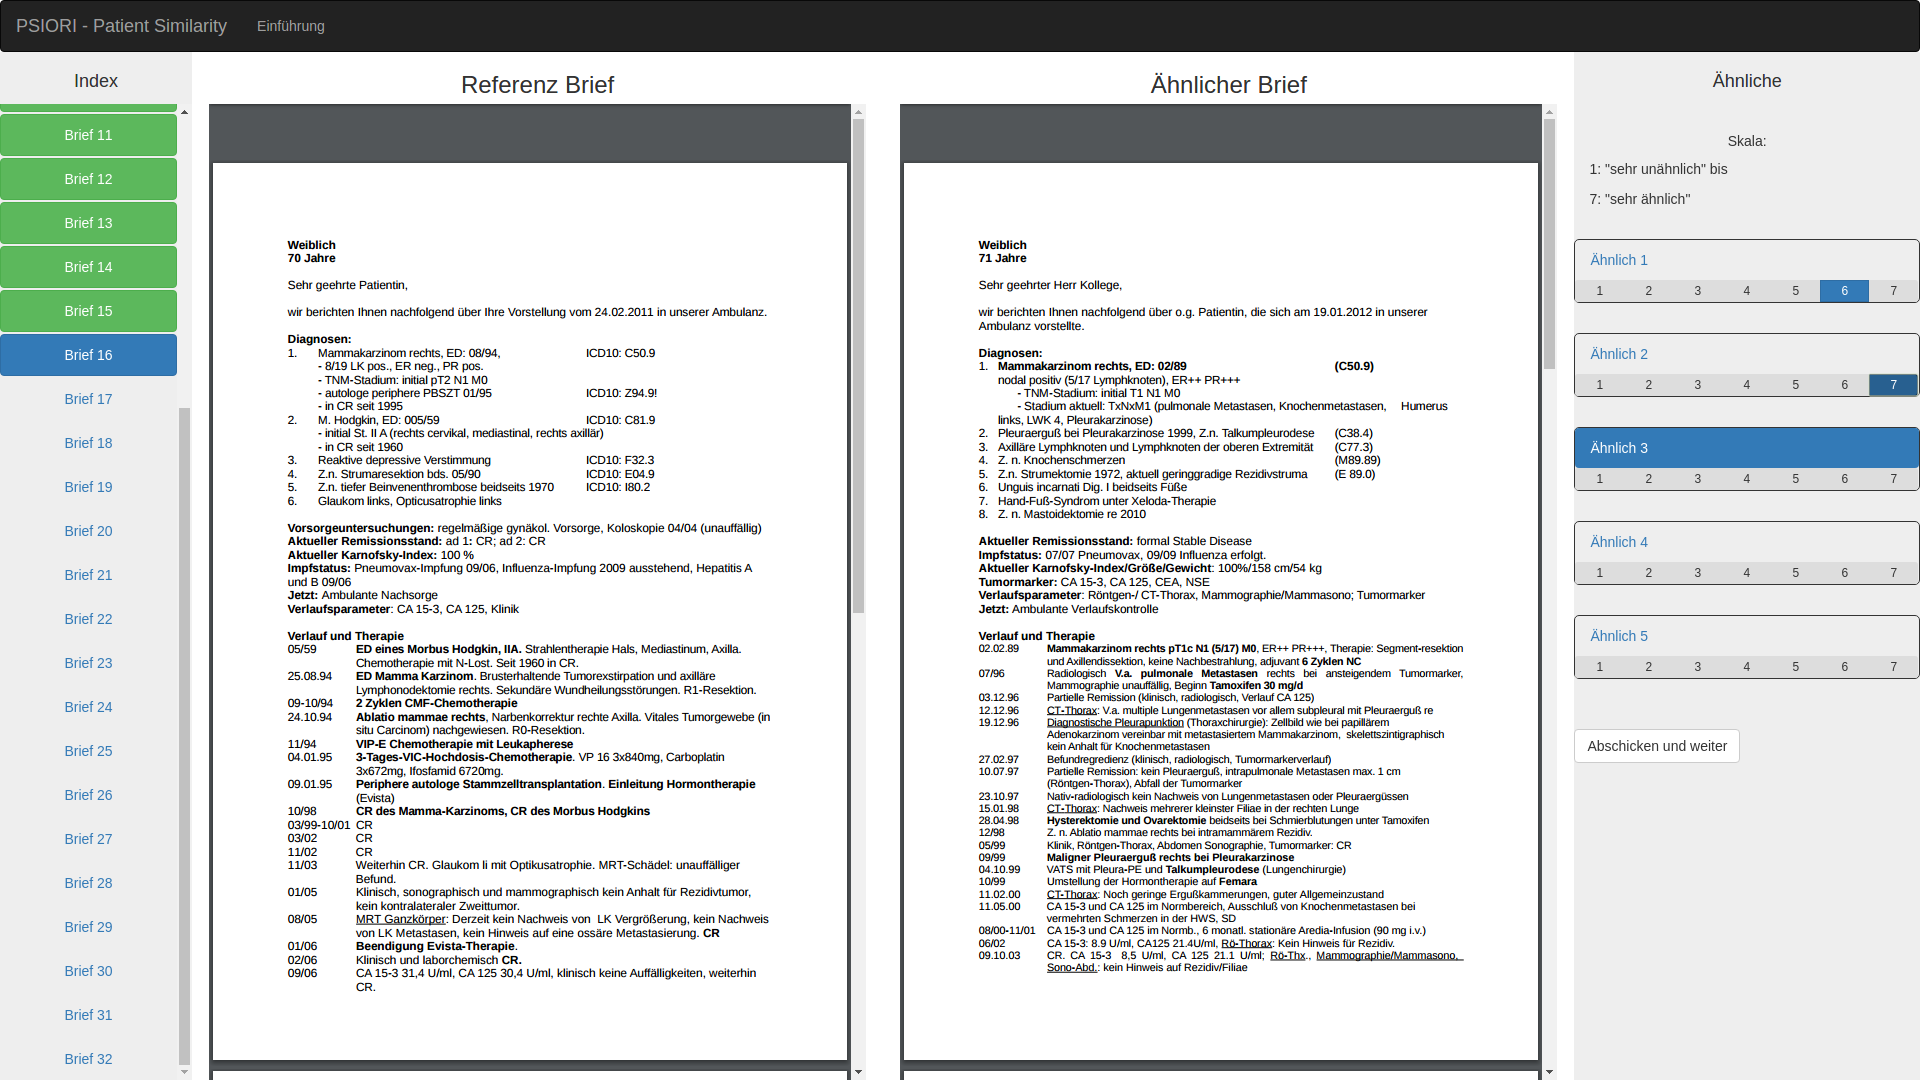
\includegraphics[width=\linewidth]{figures/webexperiment_screenshot2}
%	\caption{Screenshot of the website view during the experiment.}
%	\label{fig:webexperiment}
%\end{figure}



%We probe the similarity ratings that subjects give to pairs of letters and compare them to the similarity measure of our algorithm. We select 32 letters out of our database, 16 of them have a follow-up letter in our database, the other 16 are randomly selected among the ones without follow-up letter. We take these 32 as reference letters and select to each of them five other, so called comparison letters, with which they will be compared for similarity. Four of these five are the ones with highest cosine similarity to the reference letter as computed with our algorithm. The fifth is randomly selected and then fixed. Subjects are presented with a reference letter and the five comparison letters in a random, but fixed sequence. They are forced to give a rating for each pair in the range of 1 (very dissimilar) to 7 (very similar) and can then move on to the next reference letter. See figure \ref{fig:webexperiment} for a screens hot of the website on which the subjects perform the experiment. We ensure that among the first two reference letters is one follow-up reference letter and one non-follow-up reference letter. This way subjects can adjust for the upper similarity bound of having a letter pair with both letters from the same patient. In total we obtain ratings for 160 letter pairs from each subject. However, the rating data for the first two reference letters is discarded for the later analysis, leaving 150 letter pairs for evaluation. Six subjects perform our experiment, four experts (oncologists with at least five years of practical experience) and two novices (medical students more than halfway through their study course).



\subsection*{Results}
We first analyze whether our recommending method performs significantly better than guessing. Therefore we compare the rating of the comparison letter with highest cosine similarity to the rating of the randomly chosen comparison letter for each trial. Through bootstrapping Note that we exclude data of follow-up pairs for analysis, except where explicitly stated. Subjects rate the similarity of these pairs very highly and almost any information retrieval system will find them to be similar. Thereby they would improve positive correlation statistics in our analysis, although retrieving them is useless in practice. We will show later that our recommender can easily distinguish them from normal pairs.

We first analyze the relationship of the cosine similarity and the average subject ratings of letter pairs. The data shows a clear positive correlation of those variables (p-value: $5.0\cdot10^{-16}$), suggesting that our recommendation method captures at least some aspects of perceived similarity. See figure \ref{fig:sim_vs_rating} for a visualization of the cosine similarity as a function of the average rating of subjects.



\begin{figure}
	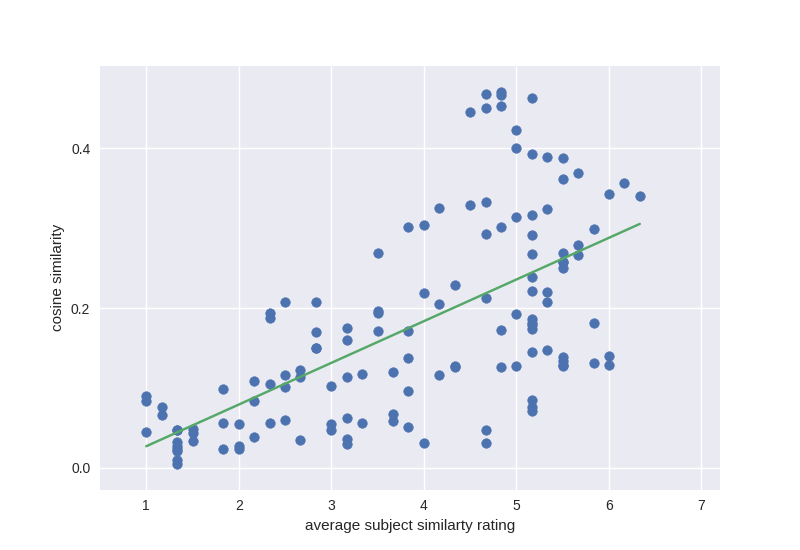
\includegraphics[width=\linewidth]{figures/similarity_vs_rating}
	\caption{Cosine similarity of letter pairs as a function of the average rating, that subjects assigned to the pair.}
	\label{fig:sim_vs_rating}
\end{figure}

\end{document}